% \iffalse meta-comment
% (c) 2021 Vincent Kuhlmann
% 
% \fi
% \iffalse
%<*driver>
\ProvidesFile{highlightlatex.dtx}[2021/03/17 highlightlatex v1.0.0 + Dev]
\NeedsTeXFormat{LaTeX2e}[1994/06/01]
\documentclass{ltxdoc}

\usepackage[margin=2.54cm]{geometry}
\usepackage{graphicx}
\usepackage{parskip}
\usepackage{listings}
\usepackage{adjustbox}
\usepackage{soul}
\usepackage{hyperref}

\iftrue \iffalse Use own package\fi
    \usepackage{highlightlatex}
    \updatehighlight{
    	name = default,
    	add = {
    		\defaultgobble
	    },
    	name = hll,
    	color = orange!90!black,
    	add = {
    		\hll, highlightblock
    	},
    	name = vert,
    	color = red,
    	add = {
    		|	
	    }
	}   
\else
    \let\hll\lstinline
    \lstnewenvironment{highlightblock}[1][]
    {%
        \lstset{#1}%
    }{}%
    \lstset{tabsize=2}
\fi

\begin{document}
    \DocInput{\jobname.dtx}
\end{document}
%</driver>
% \fi
% 
% \title{Highlight \LaTeX{} manual}
% \author{%
%    Vincent Kuhlmann\\
%     \texttt{vincent.kuhlmann@hotmail.com}
% }
%
%
% \maketitle
% \begin{abstract}
%    This package provides colored syntax highlighting for \LaTeX{} source code
%    within \LaTeX. This is in response to the trend of people often falling back
%    to very rudimentary solutions, like verbatim, to display code. For this, it
%    builds further on the generic `listings' package.
% \end{abstract}
% 
% \begin{figure}[htbp]
%     \centering
%   \rule{2cm}{1pt}
%
%    \medskip
%     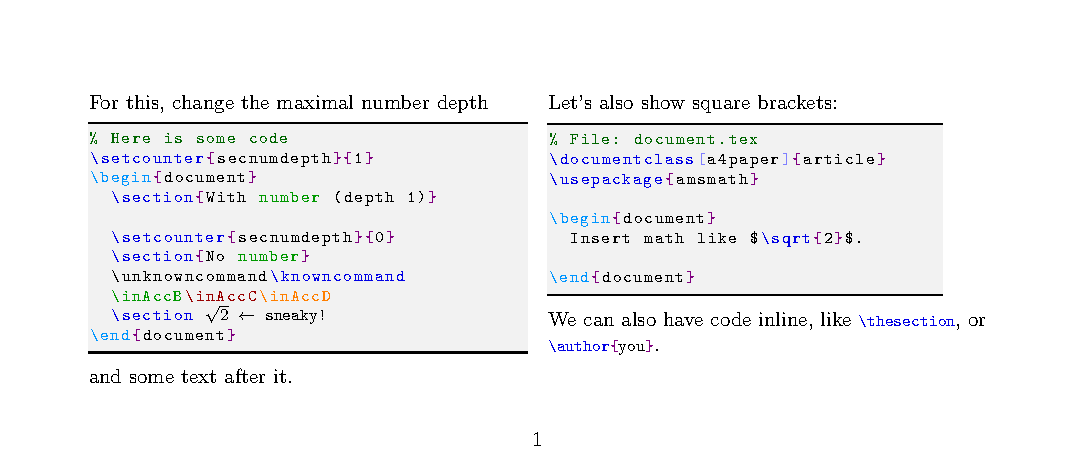
\includegraphics[width=0.9\textwidth,trim=1cm 1cm 1cm 1cm, clip]{demo.pdf}
%     \caption{Output of `demo.tex'.}
%    \rule{2cm}{1pt}
% \end{figure}
% 
% 
% \section{Example}
% \meaning\ifsomevar

% \begin{macro}{\mymacro}
%     someTest
% \end{macro}

% \DescribeEnv{myenv}
% aaa
% 
%
% some paragraph
% 
% another
% 
% 
% \section{Getting started}
% 
% After having added the package, you can add LaTeX in two ways.
% 
% \subsection{Inline style}
% 
% 
% \hspace{0.1\textwidth}%
% \adjustbox{raise=-6pt,lap=-\width}{\setulcolor{red}\ul{\textsc{example}}\;}%
% \begin{minipage}[t]{0.8\textwidth}%
% \begin{highlightblock}[gobble=6]
%      Your file begins with a line of the form \hll~{}~|\documentclass[]{}|. The
%      square brackets ...
% \end{highlightblock}
% \end{minipage}
% 
% 
% The first non-space character following \lstinline|\hll| delimits the argument to
% this command.
% 
% \subsection{Block style}
% 
% \hspace{0.1\textwidth}%
% \adjustbox{raise=-6pt,lap=-\width}{\setulcolor{red}\ul{\textsc{example}}\;}%
% \begin{minipage}[t]{0.8\textwidth}%
% \begin{highlightblock}[gobble=5]
%     Your basic document now looks like
%     \begin{highlightblock}[gobble=2]
%           \documentclass[a4paper]{article}
%           \begin{document}
%               Hello world!
%           \end{document}
%     \end{~{}~highlightblock}
% \end{highlightblock}
% \end{minipage}
% 
% To prevent indentation of our \hll|highlightblock| (here one tab) to be shown as
% part of the code, the \hll|gobble| parameter strips them off. Play around with it
% until everything looks right. I recommend to set this value globally using
% \hll|\def\defaultgobble{2}|. You can still override it on a per-block basis, if
% necessary.
% 
% There are situations where width of the block could run out of the page. For
% example, when using beamer and storing a block as described in the section
% `Fragile breaking situations', the normal full-width of a slide is assumed.
% If you use multiple columns, set the \hll|linewidth| on the \hll|highlightblock|.
% This can be a fraction of the total slide width available, \hll|0.6\textwidth|
% is 60\% of the width, or an absolute value, like \hll|10em|, which seems to equal
% 20 characters.
%
% \iffalse
% There are more keys you can provide. Check the
% [listings package documentation](https://www.ctan.org/pkg/listings) for
% options available to the `lstlisting`-environment and `lstset` command.
% 
% ## Adding a command to a highlighting rule
% 
% By default, only some LaTeX commands will be highlighted in blue. If there are
% others you need, like `\tableofcontents` and `\figref`, update the highlighting
% rules:
% ```
% \updatehighlight{
%     name = default,
%     add = {
%         \tableofcontents, \figref
%     }
% }
% ```
% 
% The change will only affect code after it. I recommend issuing `updatehighlight`
% in your preamble (before the `\begin{document}`). In some situations you might
%     want to change things mid-document. That's possible too.
%     
%     ## Custom highlighting rules
%     
%     As shown in `demo.tex`, you can put any command or keyword you want to highlight
%     in a different color. You do this with
%     ```
%     \updatehighlight{
%         % name: How you like to refer to it. Allows you to modify the style later.
%         name = spotlight,
%         color = orange,
%         add = {
%             \tableofcontents
%         }
%     }
%     ```
%     
%     You can use the `xcolor` syntax for describing colors as well. If you find the
%     orange too bright, you can replace it with `orange!90!black`: 90% orange,
%     remaining is black. For more information on color definitions and name, refer to
%     [LaTeX/Colors on Wikibooks](https://en.wikibooks.org/wiki/LaTeX/Colors).
%     
%     ---
%     
%     The argument to `\updatehighlight` is a key-value list. Keys are processed
%     sequentially. For example, use `color` before rather than after the `add`, and
%     a key can appear multiple times. Each one will be processed. You can merge any
%     two `\updatehighlight` in one. No need to close and reopen `\updatehighlight`
%     for each highlighting rule.
%     
%     You might be tempted to add a blank line for clarity; that means a new paragraph
%     to LaTeX, don't do it. Instead, just put a line with only a `%` sign. Spacing
%     within the argument is often irrelevant. If you need a comma in the value,
%     surround your value with braces.
%     
%     The possible keys are:
%     
%     * **name**: Create or modify a named rule. This key is optional.
%     
%     The default keys are `default`, which includes a bunch of basic commands,
%     and has by default a dark blue color, and `structure`, which consists of
%     `\begin` and `\end` and prints them in light blue.
%     
%     * **classoffset**: Set the `listings` classoffset manually. Try to avoid this.
%     Use **name** to refer to existing rules instead.
%     
%     * **add**: Add a commands (`\mycommand`) oor keywords (`Hi!`) to the current
%     rule. The value can contain multiple values by opening braces, and comma
%     separating values within them.
%     
%     * **remove**: Remove a commands or keywords from the current rule. The value can
%     contain multiple values by opening braces, and comma separating values within
%     them.
%     
%     * **clear**: Remove all commands and keywords from the current rule. Use without
%     value, for example
%     
%     \updatehighlight{
%         name = default,
%         clear
%     }
%     
%     * **color**: Specify a color for the rule. Equivalent to specifying **style**
%     instead, with value `\color{value}` where `value` is the value for the
%     **color** key. So `color=red` and `style=\color{red}` are equivalent.
%     
%     * **style**: Specify a style for the rule. A rule can only have one style. If
%     you specify a style after `add` or `remove`, this starts a new (unnamed) rule.
%     In practice, the only style which will probably work for you is just a color.
%     For that, using the 'color' key is just a bit easier and neater.
%     But hey, you have the option to set whatever style you want. :)
%     
%     ## Global settings
%     There are some global parameters involved in the appearance:
%     ```
%     \colorlet{curlyBrackets}{red!50!blue}
%     \colorlet{squareBrackets}{blue!50!white}
%     \colorlet{codeBackground}{gray!10!white}
%     \colorlet{comment}{green!40!black}
%     \def\defaultgobble{0}
%     ```
%     
%     Each line can be set independent of each other, and each shows its default
%     value.
%     
%     There are package options you can use as well:
%     
%     * **frame** (default: `lines`): specify the frame you want around code. My
%     favorites are `lines` and `none`. Check the
%     [listings package documentation](https://www.ctan.org/pkg/listings) for all
%     possibilities.
%     
%     * **noframe** (use without value): equivalent to `frame=none`.
%     
%     * **styleanywhere** (use without value): override the default behavior that
%     `style` starts a new style after commands like `add` and `remove`.
%     
%     ## Fragile breaking situations (like beamer frames)
%     
%     When passing command arguments around, or storing environment content, LaTeX
%     interprets all characters. This includes seeing `\maketitle` in
%     `\hll|\maketitle|` as a real command. To prevent this behavior, everything from
%     `\verb`, to the `verbatim`-environment, to the `listings` package the highlight
%     LaTeX package uses temporarily changes the interpretation of characters that are
%     still to be read. The blackslash before maketitle in `\hll|\maketitle|` will be
%     read as 'just text' (a _letter_ technically).
%     
%     When content has already been interpreted, like the `frame`-environment in
%     `beamer` does, this trick can't be done anymore. Instead, you either need to
%     _escape_ code, or _pre-process_ the code outside a fragile breaking situation.
%     
%     Escaping is done by preceding the special character with a backslash. For
%     example, `\hll|\documentclass[]{}|` becomes `\hll|\\documentclass[]\{\}|`.
%     
%     For large code blocks, this is undesirable. Therefore, the package provides for
%     a companion to the `highlightblock`-environment: surround it with a `saveblock`
%     environment which takes a single argument: a name to assign it. We use it to
%     refer to it later. For example:
%     ```latex
%     \begin{saveblock}{basicfigure}
%         \begin{highlightblock}[linewidth=0.6\textwidth]
%             \begin{figure}
%                 \includegraphics
%                 [width=0.9\linewidth]
%                 {myPlot.pdf}
%                 
%                 \caption{My plot}
%                 \label{fig:myplot}
%             \end{figure}
%         \end{highlightblock}
%     \end{saveblock}
%     ```
%     
%     Do this outside a fragile breaking situation. (For the `frame`-environment
%     example, that means just before the `frame` for example.) Then, where you want
%     to use it, use `\useblock{basicfigure}`. There is also a variant
%     `\consumeblock{basicfigure}`. If you save many blocks, these will all remain
%     loaded in memory till your PDF has fully generated. The `\consumeblock` works
%     like `\useblock`, except the saved block is deleted from memory after its use.
%     Note this can also result in unexpected behavior, for example animations in a
%     beamer frame might need the code line to be executed multiple times. Use
%     `\useblock` when you can't make the guarantee the last use of a block.
%     
%     There is a separate demo for fragile breaking situations. You can find it at
%     `deamerdemo/deamerdemo.tex`.
%     
%     ## Adding extra space
%     
%     By default, highlight-latex follows an approach where it minimizes spacing.
%     This gives you full control over how tight or spacious your document looks.
%     Just use commands like `\medskip` to add extra spacing. The package doesn't
%     currently include an option to do it everywhere automatically.
%     
%     ## License
%     
%     The package is available under MIT License. See LICENSE.txt.
%     
%     ## Credits
%     
%     Thanks for minor fixes:
%     
%     gemmaro
%     
%     ---
%     
%     For any small fix, bug, feature request, unclarity etc., you're welcome to
%     open an issue on
%     
%     [https://github.com/vkuhlmann/highlight-latex/issues](https://github.com/vkuhlmann/highlight-latex/issues)
%     
%     Thanks for thinking along!
%
% \fi
% 
% \Finale
%
\endinput
